\chapter{Ergebnisse}
In diesem Kapitel werden die Ergebnisse der zwei Modi vorgestellt. Zum einen ist dies der Offline-Modus, zum anderen der Online-Modus. 

\section{Offline-Modus}
Im Offline-Modus können mittels Kreuzvalidierung geeignete Ergebnisse erzeugt werden. Somit dient der Offline-Modus um die verschiedenen eingesetzten Algorithmen zu vergleichen. Im folgenden werden zuerst die Standardwerte, mit denen die Tests durchgeführt werden, erläutert. Dann werden die Algorithmen verglichen. Und zuletzt wird auf die Ergebnisse der Optimierung durch den Evolutionären Algorithmus eingegangen.

\subsection{Standardwerte}
Bei den Tests handelt es sich jeweils um eine Kreuzvalidierung mit drei Blöcken. Dabei kommen zehn verschiedene Sprecher zum Einsatz. Die restlichen Einstellungen können der Tabelle \ref{tbl:standardwerte} entnommen werden.

% table settings
\setlength{\tabcolsep}{10pt} %Abstand zwischen Spalten
\renewcommand{\arraystretch}{1.25} %Zeilenabstand

\begin{table}[h]
	\centering
	\label{tbl:standardwerte}
	\begin{tabular}{l|c|c|c|c}			
		& \textbf{LPC} & \textbf{MFCC} & \textbf{Neural Gas} & \textbf{SVM} \\
		\hline
		\textbf{Fensterbreite} & 32 ms & 32 ms & & \\
		\textbf{Überlappung der Fenster} & 50 \% & 50 \% & & \\
		\textbf{Minmales Energielevel} & 90 \% & 90 \% & & \\
		\textbf{Merkmale pro Fenster} & 12 & 20 & & \\
		\textbf{Fensterfunktion} & Hamming & Hamming & & \\
		\textbf{Anzahl der Prototypen} & & & 100 & \\
		\textbf{Anzahl der Iterationen} & & & 15 & \\
		\textbf{$\gamma$ und c} & & & & 1 \\
	\end{tabular}
	\caption{Standardeinstellungen der vier zu vergleichenden Algorithmen}
\end{table}

\subsection{Vergleich der Algorithmen}
Bei dem Test mit den oben genannten Standardwerten, werden die in Tabelle \ref{tbl:vergleich} aufgeführten Ergebnisse erzielt. Hierbei handelt es sich um die Erkennungsrate auf Einzelframes. Spaltenweise wird zwischen den Preprocessing-Algorithmen LPC und MFCC unterschiedenen, zeilenweise zwischen den Trainings-Algorithmen Neural Gas und SVM. Wobei bei SVM nochmals unterschieden wird zwischen dem Einsatz eines linearen Kernels und eines RBF-Kernels. Mit 80 \% Erkennungrate auf Einzelframes das beste Ergebniss erzielt die Kombination aus MFCC und SVM mit RBF-Kernel.

\begin{table}[h]
	\centering
	\label{tbl:vergleich}
	\begin{tabular}{l|c|c}			
		& \textbf{LPC} & \textbf{MFCC} \\
		\hline
		\textbf{Neural Gas} & 40 \% & 71 \% \\
		\textbf{SVM (linearer Kernel)} & 46 \% & 72 \% \\
		\textbf{SVM (RBF-Kernel)} & 54 \% & 80 \% \\
	\end{tabular}
	\caption{Erkennungsrate auf Einzelframes}
\end{table}

Im den Abbildungen TODO werden Verwechlsungsmatrixen einiger Kombinationen aufgezeigt. Jeweils in der linken Hälfte sind die Anzahl der Erkennungen in Prozentzahlen und rechts daneben die visuelle Darstellung derselben. Auf der x-Achse ist jeweils der erkannte Sprecher, auf der y-Achse der tatsächliche Sprecher aufgetragen. Ideal wären also Matrixen mit 100 \% bzw. die dazu passenden Kreise auf der Diagonale.

% table settings
\setlength{\tabcolsep}{6pt} %Abstand zwischen Spalten
\renewcommand{\arraystretch}{1.1} %Zeilenabstand

\begin{figure}[h]
	\label{tbl:lpcNgMatrix}
	\centering
	\hspace*{-15mm}
	\begin{minipage}[t]{0.58\linewidth}
		\begin{tabular}{c|cccccccccc}
			& \textbf{1} & \textbf{2} & \textbf{3} & \textbf{4} & \textbf{5} & \textbf{6} & \textbf{7} & \textbf{8} & \textbf{9} & \textbf{10} \\ \hline
			\textbf{1} & 54 & 6 & 4 & 3 & 6 & 4 & 5 & 3 & 12 & 2 \\
			\textbf{2} & 5 & 50 & 8 & 4 & 8 & 3 & 9 & 5 & 6 & 3 \\
			\textbf{3} & 6 & 12 & 29 & 7 & 10 & 6 & 8 & 11 & 4 & 7 \\
			\textbf{4} & 5 & 6 & 7 & 65 & 3 & 1 & 1 & 5 & 3 & 5 \\
			\textbf{5} & 6 & 7 & 7 & 2 & 26 & 9 & 16 & 10 & 9 & 9 \\
			\textbf{6} & 4 & 2 & 5 & 1 & 9 & 31 & 13 & 13 & 14 & 9 \\
			\textbf{7} & 3 & 8 & 3 & 1 & 12 & 10 & 27 & 12 & 8 & 16 \\
			\textbf{8} & 3 & 4 & 6 & 3 & 10 & 10 & 14 & 27 & 8 & 14 \\
			\textbf{9} & 10 & 7 & 4 & 2 & 8 & 14 & 9 & 10 & 33 & 5 \\
			\textbf{10} & 1 & 1 & 2 & 2 & 4 & 8 & 11 & 10 & 3 & 56 \\
		\end{tabular}
	\end{minipage}
	\begin{minipage}[t]{0.4\linewidth}
		\centering
    	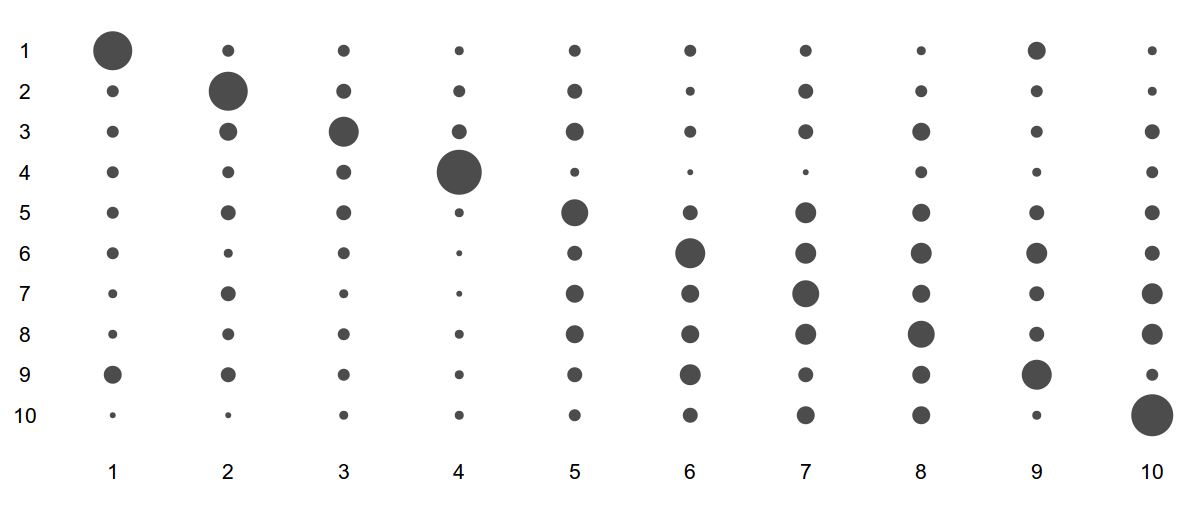
\includegraphics[width=1\linewidth]{images/lpcNgMatrix}
	\end{minipage}
	\caption{Verwechslungsmatrix für die Kombination LPC und Neural Gas}
\end{figure}

TODO weitere Verwechslungsmatrixen und das saubere Anordnen nebeneinander...
		
\subsection{Optimierung durch Evolutionären Algorithmus}
Es wird das Maximum in einem 6-dimensionale Vektorraum, der sich durch die verschiedenen Parameter von MFCC und Neural Gas ergeben, mittels eines Evolutionären Algorithmus gesucht. Hierbei wird die Fitnessfunktion \ref{equ:fitness} maximiert. In die Fitnessfunktion gehen die Erkennungsrate (engl. \emph{accuracy}) und die Dauer (engl. \emph{duration}) des Individuums ein. In Abbildung \ref{fig:ea1} sind diese drei Punktdiagramme eingezeichnet. Die Schwankungen, die darin zu sehen sind, sind gewollt und erhöhen die Diversität.

\begin{figure}[h]
	\label{fig:ea1}
	\centering
	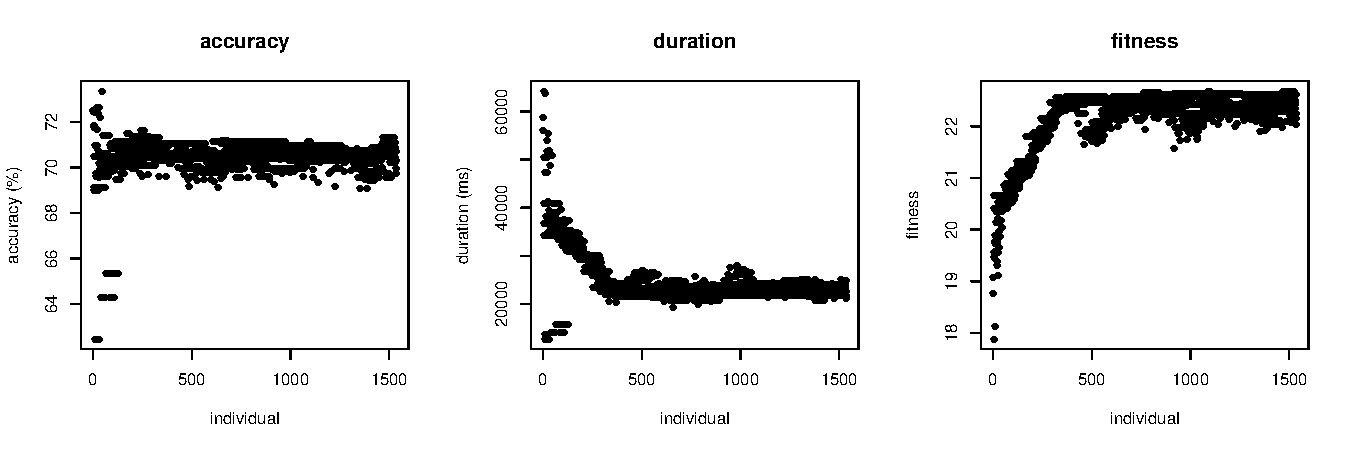
\includegraphics[width=1\textwidth]{images/ea1}
	\caption{Erkennungsrate, Dauer und die dazugehörige Fitness}
\end{figure}

Um nun das Optimum sowohl was die Dauer der Ausführung, als auch der Erkennungsrate angeht, zu finden, wird eine Pareto-Front erstellt. Diese ist in Abbildung \ref{fig:ea2} dargestellt. Grün dargestellte Punkte stellen die Pareto-Front dar.

\begin{figure}[h]
	\label{fig:ea2}
	\centering
	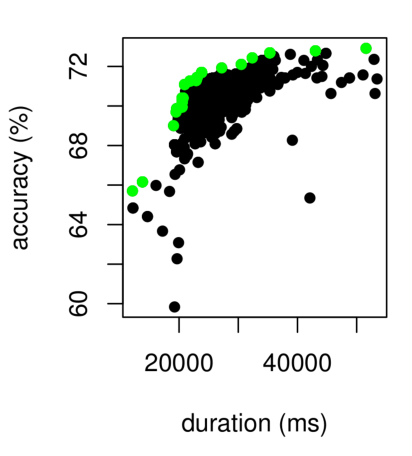
\includegraphics[width=0.5\textwidth]{images/ea2}
	\caption{Pareto-Front (grüne Punkte)}
\end{figure}

Hieraus ergeben sich folgende optimale Werte für MFCC und Neural Gas. Überlappen sich die Fenster bis zu 80 \% kann eine bessere Erkennungrate erzielt werden, allerdings erhöht sich auch die Ausführungsdauer. Wobei auch schon mit geringer oder gar keiner Überlappung beachtliche Erkennungsraten erreicht werden. Das optimale Energielevel liegt zwischen 96 \% und 85 \%. Die niedrigeren Energielevel haben eine bessere Erkennungsrate zur Folge. Die optimale Anzahl von Merkmalen der Feature Vektoren schwankt zwischen 25 und 33 Stück. Bei Neural Gas liegen die Anzahl der Prototypen zwischen 53 und 176 Stück. Höhere Prototypenanzahlen haben bessere Erkennungsraten, aber auch schlechtere Ausführungsgeschwindigkeiten zur Folge. Das gleiche gilt für die Anzahl der Iterationen des Algorithmus. Wobei hier die Spanne zwischen 5 und 9 Iterationen liegt.

Folglich hat die Parameteroptimierung die Erkennungsrate nochmals um ca. zwei Prozentpunkte gegenüber der Erkennungsrate mit den Standardparametern erhöht. Ob wirklich ein globales Optimum gefunden wird, kann bei einem Evolutionären Algorithmus nur schwer, meist gar nicht, bewiesen werden. Somit stellen die angegeben Werte lediglich ein in dieser Projektarbeit erreichtes Optimum dar.

\section{Online-Modus}
Da für den Online-Modus kein Testszenario vorhanden ist, sind die Ergebnisse dieses Modus nur subjektiv. Durch das implementierte Programm können nur schlechte bis mittelmäßige Erkennungsraten erzielt werden. Vieles ist von den Sprechern und den Mikrophonen abhängig. So werden manche Sprecher besser erkannt, als andere.
